\subsection{Training Setup}
\label{sec:training_setup}
For weight initialization, we follow the same settings provided in the Megatron-LM codebase,\footnote{\url{https://github.com/NVIDIA/Megatron-LM/blob/main/examples/pretrain_gpt3_175B.sh}} using a normal distribution with zero mean and standard deviation of 0.006.  Standard deviation for output layers are scaled by a $1.0/\sqrt{2 L}$ term where $L$ is the total number of layers. All bias terms are initialized as 0, and all models are trained with ReLU activation and a sequence length of 2048.

We use an AdamW optimizer \cite{AdamW} with $(\beta_1,\beta_2)$ set to $(0.9, 0.95)$, and weight decay of $0.1$.  We follow a linear learning rate schedule, warming up from $0$ to the maximum learning rate over the first 2000 steps in OPT-175B, or over 375M tokens in our smaller baselines, and decaying down to 10\% of the maximum LR over 300B tokens.  A number of mid-flight changes to LR were also required (see Section~\ref{sec:training_process}).  Our batch sizes range from 0.5M to 4M depending on the model size (see Table \ref{tab:model_sizes}) and is kept constant throughout the course of training.

We use a dropout of 0.1 throughout, but we do not apply any dropout to embeddings. We clip gradient norms at 1.0, except for some mid-flight changes that reduce this threshold down from 1.0 to 0.3 (see Section~\ref{sec:training_process}).  We also include a gradient predivide factor to reduce the risk of over/underflows when computing the gradient across all ranks (splitting the division by the world size of $N$ into two division operations by $\sqrt{N}$).

\subsection{Pre-training Corpus}
\label{sec:training_dataset}
The pre-training corpus contains a concatenation of datasets used in RoBERTa \cite{liu2019roberta}, the Pile \cite{thepile}, and PushShift.io Reddit \cite{reddit2020, roller-etal-2021-recipes}. All corpora were previously collected or filtered to contain predominantly English text, but a small amount of non-English data is still present within the corpus via CommonCrawl.

We removed duplicated documents across all datasets by filtering out documents via MinhashLSH \cite{rajaraman2011mining} with a Jaccard similarity $\geq.95$. We found the Pile was particularly full of duplicate documents, and advise future researchers using the Pile to perform additional de-duplication processing.

We tokenize all corpora using the GPT-2 byte level BPE tokenizer \cite{sennrich2016bpe,radford2019language,brown2020gpt3}. Our final corpus contains roughly 180B tokens.

\paragraph{RoBERTa} We included the BookCorpus \cite{books2015} and Stories \cite{ccstories2018} subsets of the RoBERTa corpus and utilized an updated version of CCNews, containing news stories crawled through September 28, 2021. This CCNews v2 corpus was preprocessed the same way as the original RoBERTa CCNews \cite{liu2019roberta}.

\paragraph{The Pile} We included a subset of the Pile \cite{thepile}, including: CommonCrawl, DM Mathematics,  Project Gutenberg, HackerNews, OpenSubtitles, OpenWebText2, USPTO and Wikipedia. Other subsets of the Pile were eliminated as we found they increased the risk of instabilities, as measured by tendency to cause spikes in gradient norms at the 1.3B scale, or were otherwise deemed unsuitable.  All subsets went through additional ad-hoc whitespace normalization.

\paragraph{PushShift.io Reddit} We included a subset of the Pushshift.io corpus produced by \citet{reddit2020} and previously used by \citet{roller-etal-2021-recipes}. To convert the conversational trees into language-model-accessible documents, we extracted the longest chain of comments in each thread and discarded all other paths in the tree. This reduced the corpus by about 66\%.


\subsection{Training Efficiency}
\label{sec:training_efficiency}
We trained \OPT{} on 992 80GB A100 GPUs, by utilizing Fully Sharded Data Parallel \cite{1TMoE2021} with Megatron-LM Tensor Parallelism \cite{shoeybi2019megatron}. We achieve utilization of up to 147 TFLOP/s per GPU. We keep Adam state in FP32, since we shard it across all hosts, while the model weights remained in FP16. To avoid underflows, we used dynamic loss scaling, as described in \citet{micikevicius2017mixed}.


\subsection{Training Processes}
Here we describe significant training process adjustments that arose during \OPT{} pre-training.

\label{sec:training_process}
\paragraph{Hardware Failures} 
We faced a significant number of hardware failures in our compute cluster while training \OPT{}. In total, hardware failures contributed to at least 35 manual restarts and the cycling of over 100 hosts over the course of 2 months. During manual restarts, the training run was paused, and a series of diagnostics tests were conducted to detect problematic nodes. Flagged nodes were then cordoned off and training was resumed from the last saved checkpoint. Given the difference between the number of hosts cycled out and the number of manual restarts, we estimate 70+ automatic restarts due to hardware failures. 


\paragraph{Loss Divergences}
Loss divergences were also an issue in our training run. When the loss diverged, we found that lowering the learning rate and restarting from an earlier checkpoint allowed for the job to recover and continue training.  We noticed a correlation between loss divergence, our dynamic loss scalar crashing to 0, and the $l^2$-norm of the activations of the final layer spiking. These observations led us to pick restart points for which our dynamic loss scalar was still in a ``healthy'' state ($\geq1.0$), and after which our activation norms would trend downward instead of growing unboundedly.  Our empirical LR schedule is shown in Figure~\ref{fig:lr}. Early in training, we also noticed that lowering gradient clipping from 1.0 to 0.3 helped with stability; see our released logbook for exact details.
Figure~\ref{fig:validation_ppl} shows our validation loss with respect to training iterations.

\begin{figure}[t]
    \centering
    
\includegraphics[width=0.98\linewidth]{figures/lr.pdf}
    \caption{\textbf{Empirical LR schedule.} We found that lowering learning rate was helpful for avoiding instabilities.}
    \label{fig:lr}
\end{figure}

\begin{figure}
    \centering
    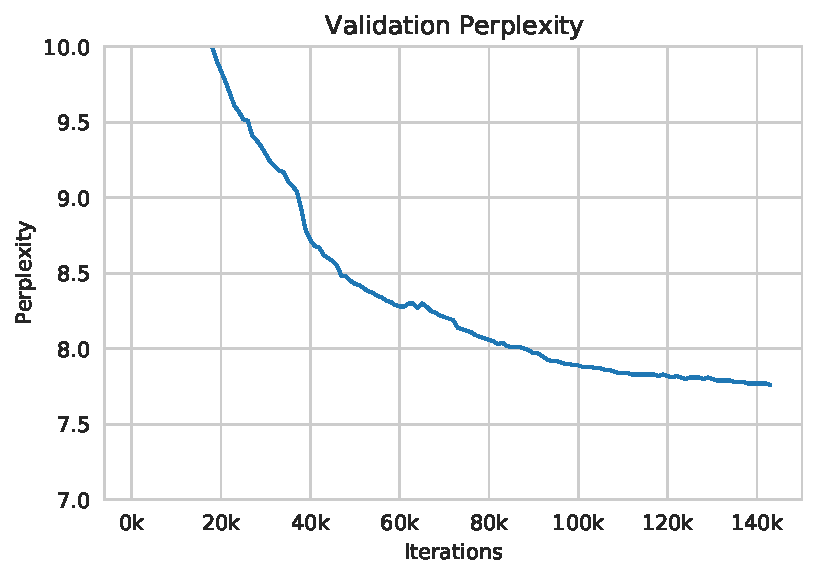
\includegraphics[width=0.98\linewidth]{figures/ppl.pdf}
    \caption{\textbf{Validation Perplexity.} Our mid-flight LR
    changes had clear effects on validation perplexity.}
    \label{fig:validation_ppl}
\end{figure}

\paragraph{Other Mid-flight Changes} 
We conducted a number of other experimental mid-flight changes to handle loss divergences. These included: switching to vanilla SGD (optimization plateaued quickly, and we reverted back to AdamW); resetting the dynamic loss scalar (this helped recover some but not all divergences); and switching to a newer version of Megatron (this reduced pressure on activation norms and improved throughput).

